In previous chapters, we dealt with methods that will produce an optimal
solution, if we provide them enough execution time. The challenge is to solve
problems with a huge amount of nodes, and for that reason, we have to drop
optimality seeking different strategies. But if we still have a feeling for
optimality, the choice is to move to approximation algorithms.

In an approximation algorithm, it is theoretical-guaranteed that the solution
is less then a factor $k$ from the optimal (since we're dealing with a
minimization problem), but the algorithm could also return a better one (even
the optimal one!).

The algorithms we're going to present works for a restricted version of the
problem: $\Delta$-TSP, in which the costs follow triangular inequality ($c_{ij}
\le c_{ik} + c_{kj},\ \forall\ i,j,k$). Since euclidean distance respect those
rule, Euclidean TSP is a restricted version of $\Delta$-TSP.

\section{$2$-approximation algorithm}
A $2$-approximation algorithm follows a simple idea: the optimal tour without an
edge, in a graph-theory point of view, is a single path visiting all the nodes.
Since that path is connected and acyclic, the path represents a spanning tree of
the nodes, which cost is greater than the shortest spanning tree (because that's
the shortest one) and less than the optimal tour (since we removed an edge).

\begin{equation*}
    cost(SST) \leq cost(path) \leq cost(optimal\ tour)
\end{equation*}

Let's now build a tour starting from the SST and doubling its edges by creating
a direct version of the tour. From that we will create a tour visiting each node
only once (a Hamiltonian cycle) by \emph{short-cutting} operation: starting
from the root node and standing on a node $a$, we will add the arc $(a,b)$ where
b is the next, unvisited node of the tour starting from $a$ or the root node if
there's no remaining node to visit. 

\begin{equation*}
    cost(tour) \leq 2 \cdot cost(SST) \leq 2 \cdot cost(optimal\ tour)
\end{equation*}

For this reason, we can talk about \emph{$2$-approximation algorithm}.

\begin{figure}[h]
    \centering
    \begin{minipage}{.3\textwidth}
        \centering
        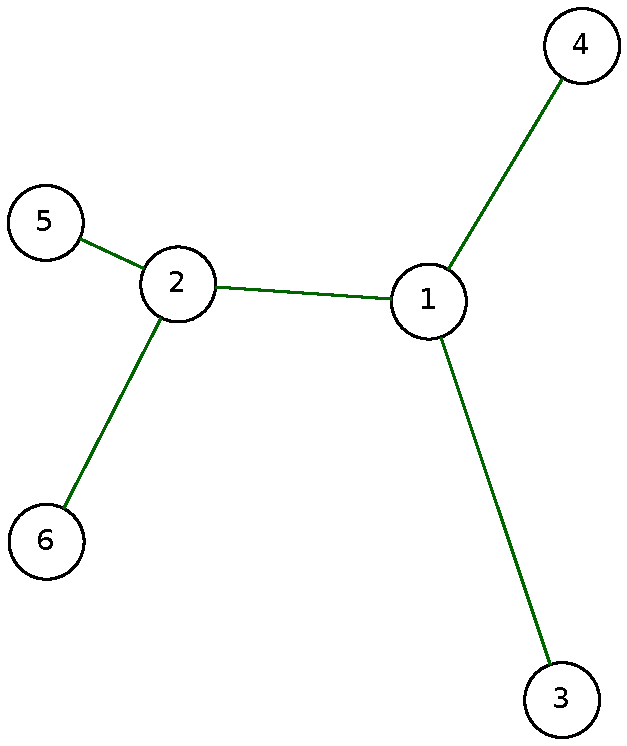
\includegraphics[width=0.8\linewidth]{figures/2approxa}
        \label{fig:sub1}
    \end{minipage}%
    \begin{minipage}{.3\textwidth}
        \centering
        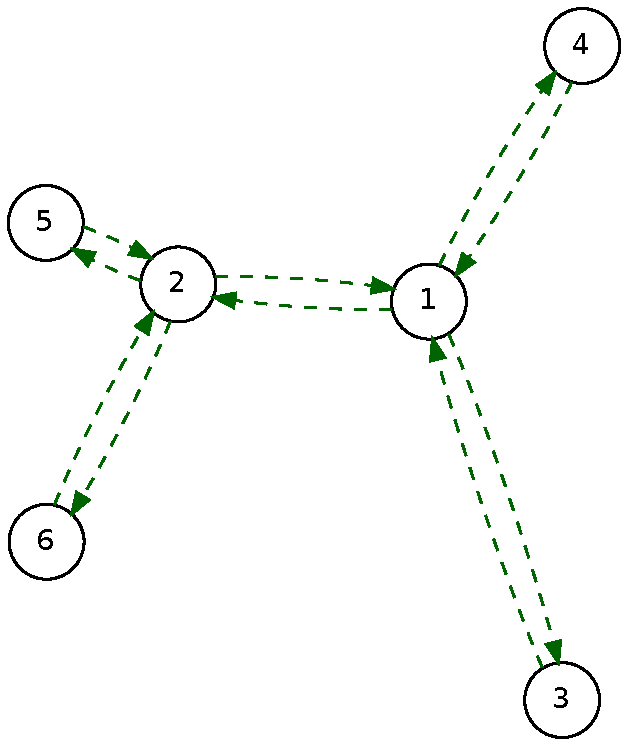
\includegraphics[width=0.8\linewidth]{figures/2approxb}
        \label{fig:sub2}
    \end{minipage}
    \begin{minipage}{.3\textwidth}
        \centering
        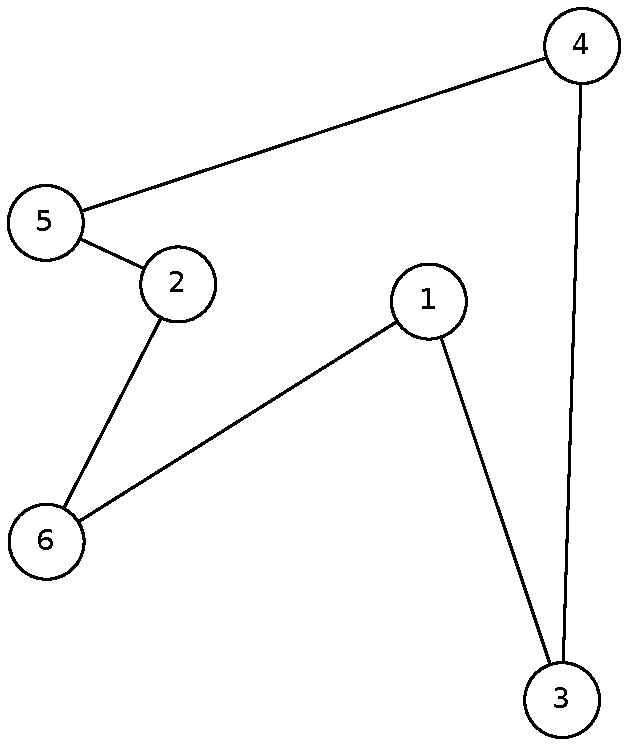
\includegraphics[width=0.8\linewidth]{figures/2approxc}
        \label{fig:sub2}
    \end{minipage}
    \caption[Shortcut example]{\centering Starting from 5 (root), the post-order visit of the tree
    is: 5 2 6 (2 skipped) 1 3 4 5}
\end{figure}

\subsection{Implementation details}
Kruskal's algorithm is implemented for the SST. Internally, it uses a
path-compressed union-find data structure mixed with classical node pointer
implementation of a tree. An additional data structure is implemented for the
visit because the union-find (especially when path compressed) doesn't track the
tree structure. In this way, both the SST computation and visit are fast
($\mathcal{O}(|V|^2log|V) + \mathcal{O}(n)$).
For this algorithm, some degree of freedom is available to tune: since an
undirected tree has no root, one may choose the node he prefers. The visit also
can be adapted, a post-order visit that starts from the union-find root has been
implemented for convenience, but a pre-order also works fine. To be honest, the
most trivial way is to topologically visit the tree starting from node 1. Both
approaches are equivalent since the theoretical guarantee is respected.
The approach is not optimal for the $\Delta$-TSP problem: some crossing may
pop out. Dealing with this kind of situation will be discussed subsequently.

Since its direct competitors will be introduced in
\autoref{chap:metaheuristics}, we're going to present results later on.

\section{$\nicefrac{3}{2}$-approximation algorithm}
A $\nicefrac{3}{2}$-approximation algorithm has been developed by Christofides,
a British mathematician in 1976. It was the best approximation algorithm for
many years, and its main idea is very similar to the one we just presented but
with a twist: the author thought that doubling the edges of the SST was too
expensive: instead of that, one could simply add some edges to the tree until an
\emph{Euler cycle} (a tour that touches each edges exactly one) has been formed.
This Euler cycle touches some nodes multiple times, and it needs to be
shortcutted to obtain a Hamiltonian cycle. The extra edges can be found
using a \emph{matching} of the graph (set of edges without common nodes) that
can be computed in polynomial time (even if $\mathcal{O}(n^3)$).

Since this algorithm is not good in practice (even considering the
theoretical guarantee), it will not be implemented.
